\documentclass{pnastwo}
\usepackage{cite}
\usepackage{color}
\usepackage{pgf}

\begin{document}

\title{Demography and selection since maize domestication}
\author{Timothy M. Beissinger\affil{1}{University of
    California,Davis}, Li Wang\affil{2}{Iowa State University}, Arun
  Durvasula\affil{1}{}, Kate Crosby\affil{1}{}, Matthew Hufford\affil{2}{}, \and Jeffrey
  Ross-Ibrarra\affil{1}{}\affil{3}{Genome Center, UC
    Davis}\affil{4}{Center for population biology, UC Davis} }

\significancetext{This work is insignificant ;-)}

\maketitle

\begin{article}

\begin{abstract}
This is the abstract. It should probably be somewhere around 200 words.
\end{abstract}

\dropcap{T}his is the beginning of the article. For now, I will give a
bulleted list of the introduction:
\begin{enumerate}
\item Maize
\item Plant domestication
\item Maize domestication
\item Importance of demography
\item Background selection
\end{enumerate}



\section{Results}
\subsection{Patterns of variability differ between genic and
  nongenic regions of the genome}
Previous research of the maize domestication process has relied upon
observations drawn from genic DNA \textcolor{red}{(several references
  here)}. Our data were generated through whole genome sequencing,
which eliminated this constraint. Importantly, we observed substantial
differences in patterns of diversity between genic and non-genic regions
of the genome for both maize and teosinte. For maize, mean pairwise
diversity ($\pi$) within genes was significantly lower than at
positions at least 5kb away from genes (0.00668 within, 0.00691 away, p$<$2e-44). The same
pattern of significantly greater diversity outside of genes was observed in
teosinte, but to a larger extent. For teosinte we observed $\pi$
within genes to be 0.0088 and at least 5kb from genes it was 0.1153
(p$\approx$0). These obserrvations suggest that genes are not evolving
neutrally in maize or teosinte. Instead, some form of selection is likely
reducing diversity within genes. Additionally, these observations
suggest that demographic inference, which relies on the assumption of
neutrally evolving DNA, will be more accurate if it is based on
observations from non-genic genetic material.

\subsection{Hard sweeps do not shape maize (or teosinte) diversity}
A mutation that is immediately beneficial and positively selected leaves a classical hard
sweep signature in the genome, whereby genetic diversity surrounding
that mutation is reduced as the haplotype where the mutation first
arose increases in frequency to fixation. The prevalence of such hard
sweeps was evaluated by comparing diversity
surrounding non-synonymous and synonymous substitutions in maize and
teosinte since divergence from tripsicum, roughly \textcolor{red}{ZZZ} years before
present \textcolor{red}{(ref here)}. For both taxa, no difference in diversity
surrounding these classes of substitutions was identified (Figure \ref{hardSweeps}). Additionally, diversity around maize substitutions
not seen in teosinte was investigated. These sites have the
potential to correspond to recent maize sweeps, occuring after the
split from teosinte. Again, no difference was observed
between diversity around synonymous and nonsynonymous
substitutions \textcolor{red}{(Supplemental figure here)}. Together, these observations suggest that hard sweeps
are not a primary form of selection for either maize or teosinte.

\begin{figure}[b]
%\vspace*{.05in}
\centering
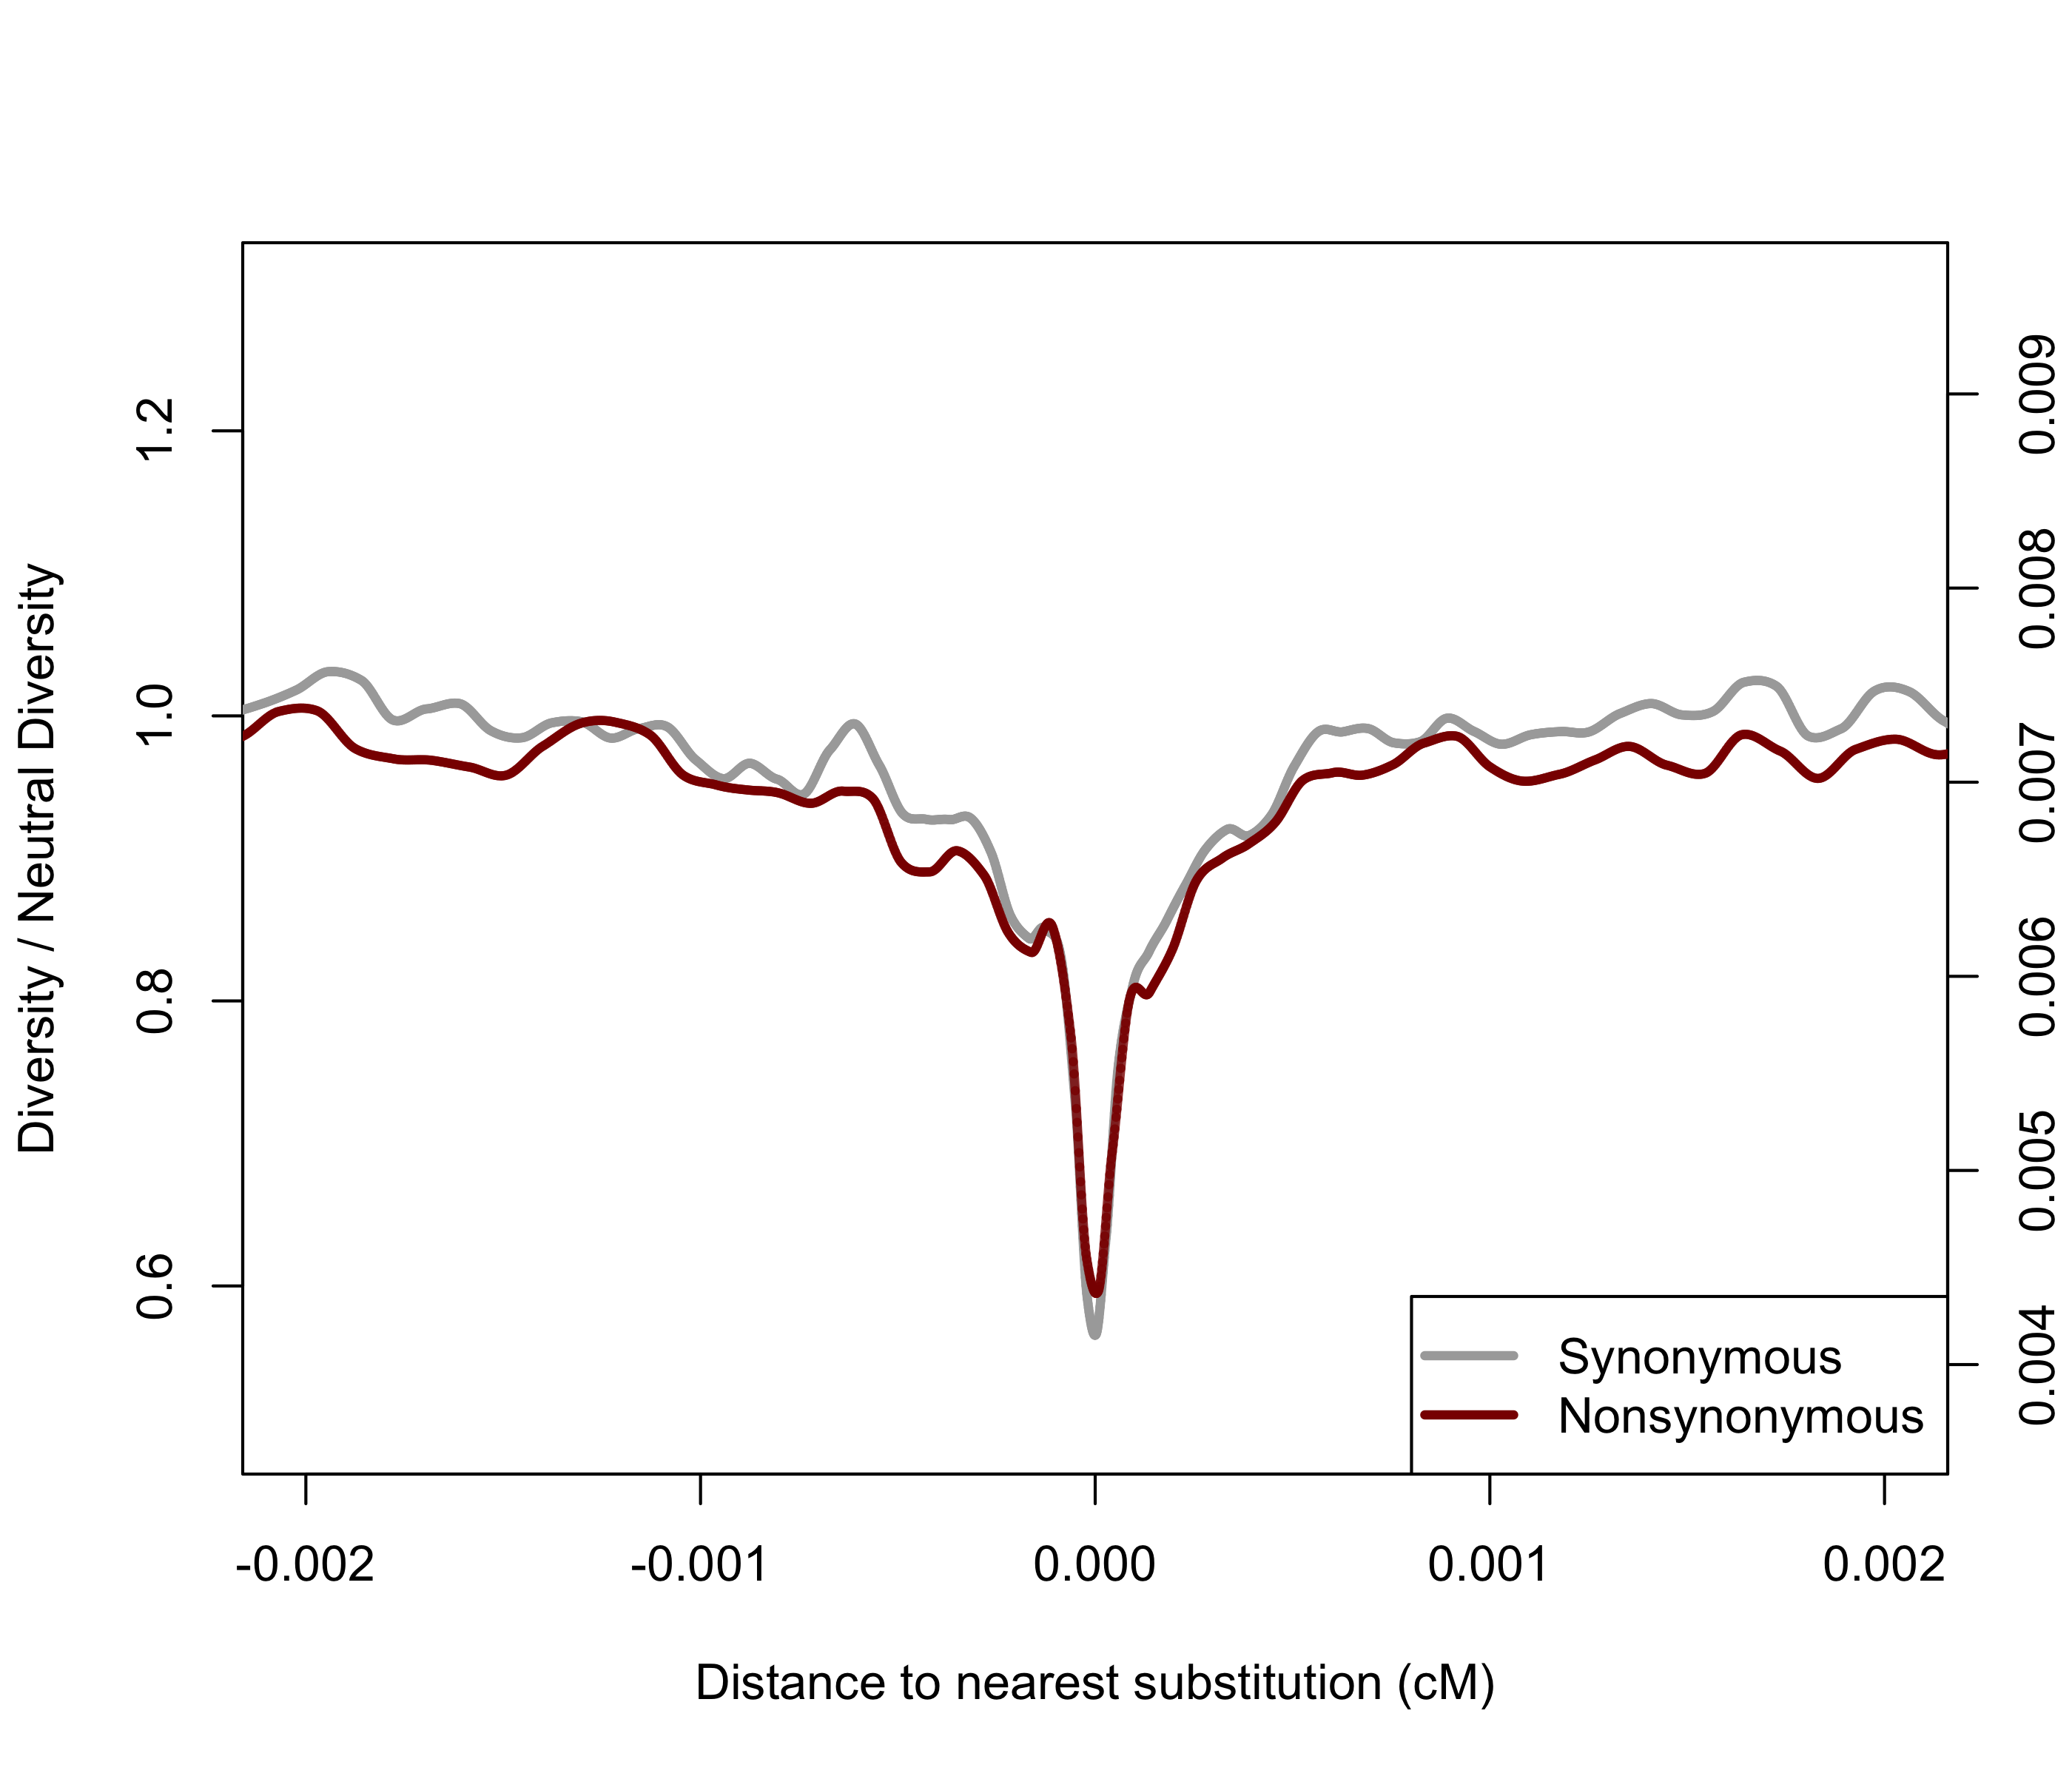
\includegraphics[width=.5\textwidth]{FigsAndFiles/plotDiversity_TvM_Folded2_unNeutralized}
\caption{Pairwise diversity surrounding synonymous and nonsynonymous
  substitutions in maize. Observe that the reduction of diversity
  surrounding nonsynonymous subsitutions is no more severe than the
  reduction of diversity surrounding synonymous substitutions. This
  equivalency suggests that hard sweeps are not a primary driver of
  maize diversity.}
\label{hardSweeps}
\end{figure}


\subsection{Patterns of purifying and background selection can be explained by demography}
Purifying selection refers to the situation where deleterious
mutations arising in a population are continuously selected against. When this
form of selection is operating, it can serve to reduce genetic
variability at linked neutral sites, a phenomenon referred called
background selection \cite{charlesworth1993}. Purifying and background selection lead
to lower diversity within genes and other functional sites relative
to neutral regions \textcolor{red}{(ref here)}. We investigated purifying
selection in maize and teosinte by evaluating the average magnitude of reduced
diversity within genes and recovery away from genes in both taxa. When standardized by neutral
levels (which we defined as diversity at least \textcolor{red}{0.01} cM distal
from genes), a stronger reduction of diversity
and slower recovery was observed for teosinte than for maize, implying
that purifying selection has left a more pronounced signature in the
teosinte genome (Figure \ref{purify}). This conflicted with our \emph{a priori} hypothesis;
we expected that strong artificial selection since domestication would
have caused enhanced purifying selection for maize. We therefore
conducted the same analysis based on singleton diversity. As a class,
singleton alleles depict the most recent patterns of evolution, but
also have the lowest effect on pairwise diversity. Therefore, unlike
pairwise diversity, patterns of singleton
diversity reflect recent patterns of evolution. When
evaluating the data in this manner, an opposite relationship was
observed. Maize singleton diversity was lower than teosinte singleton
diversity near genes, and recovered more slowly
(Figure \ref{purify}), implying that in the
recent past maize has been more influenced by purifying selection than
teosinte. Together, these findings imply that demographic history has
a strong influence on the effect of purifying selection. Historically,
teosinte has had a larger population size than maize, and only
recently has maize population size overcome that of teosinte. Since
the efficacy of purifying selection scales with population size,
these results likely reflect changes in $N_e$ more than they reflect
underlying changes in selection pressure.


\begin{figure*}[b]
%\vspace*{.05in}
\centering
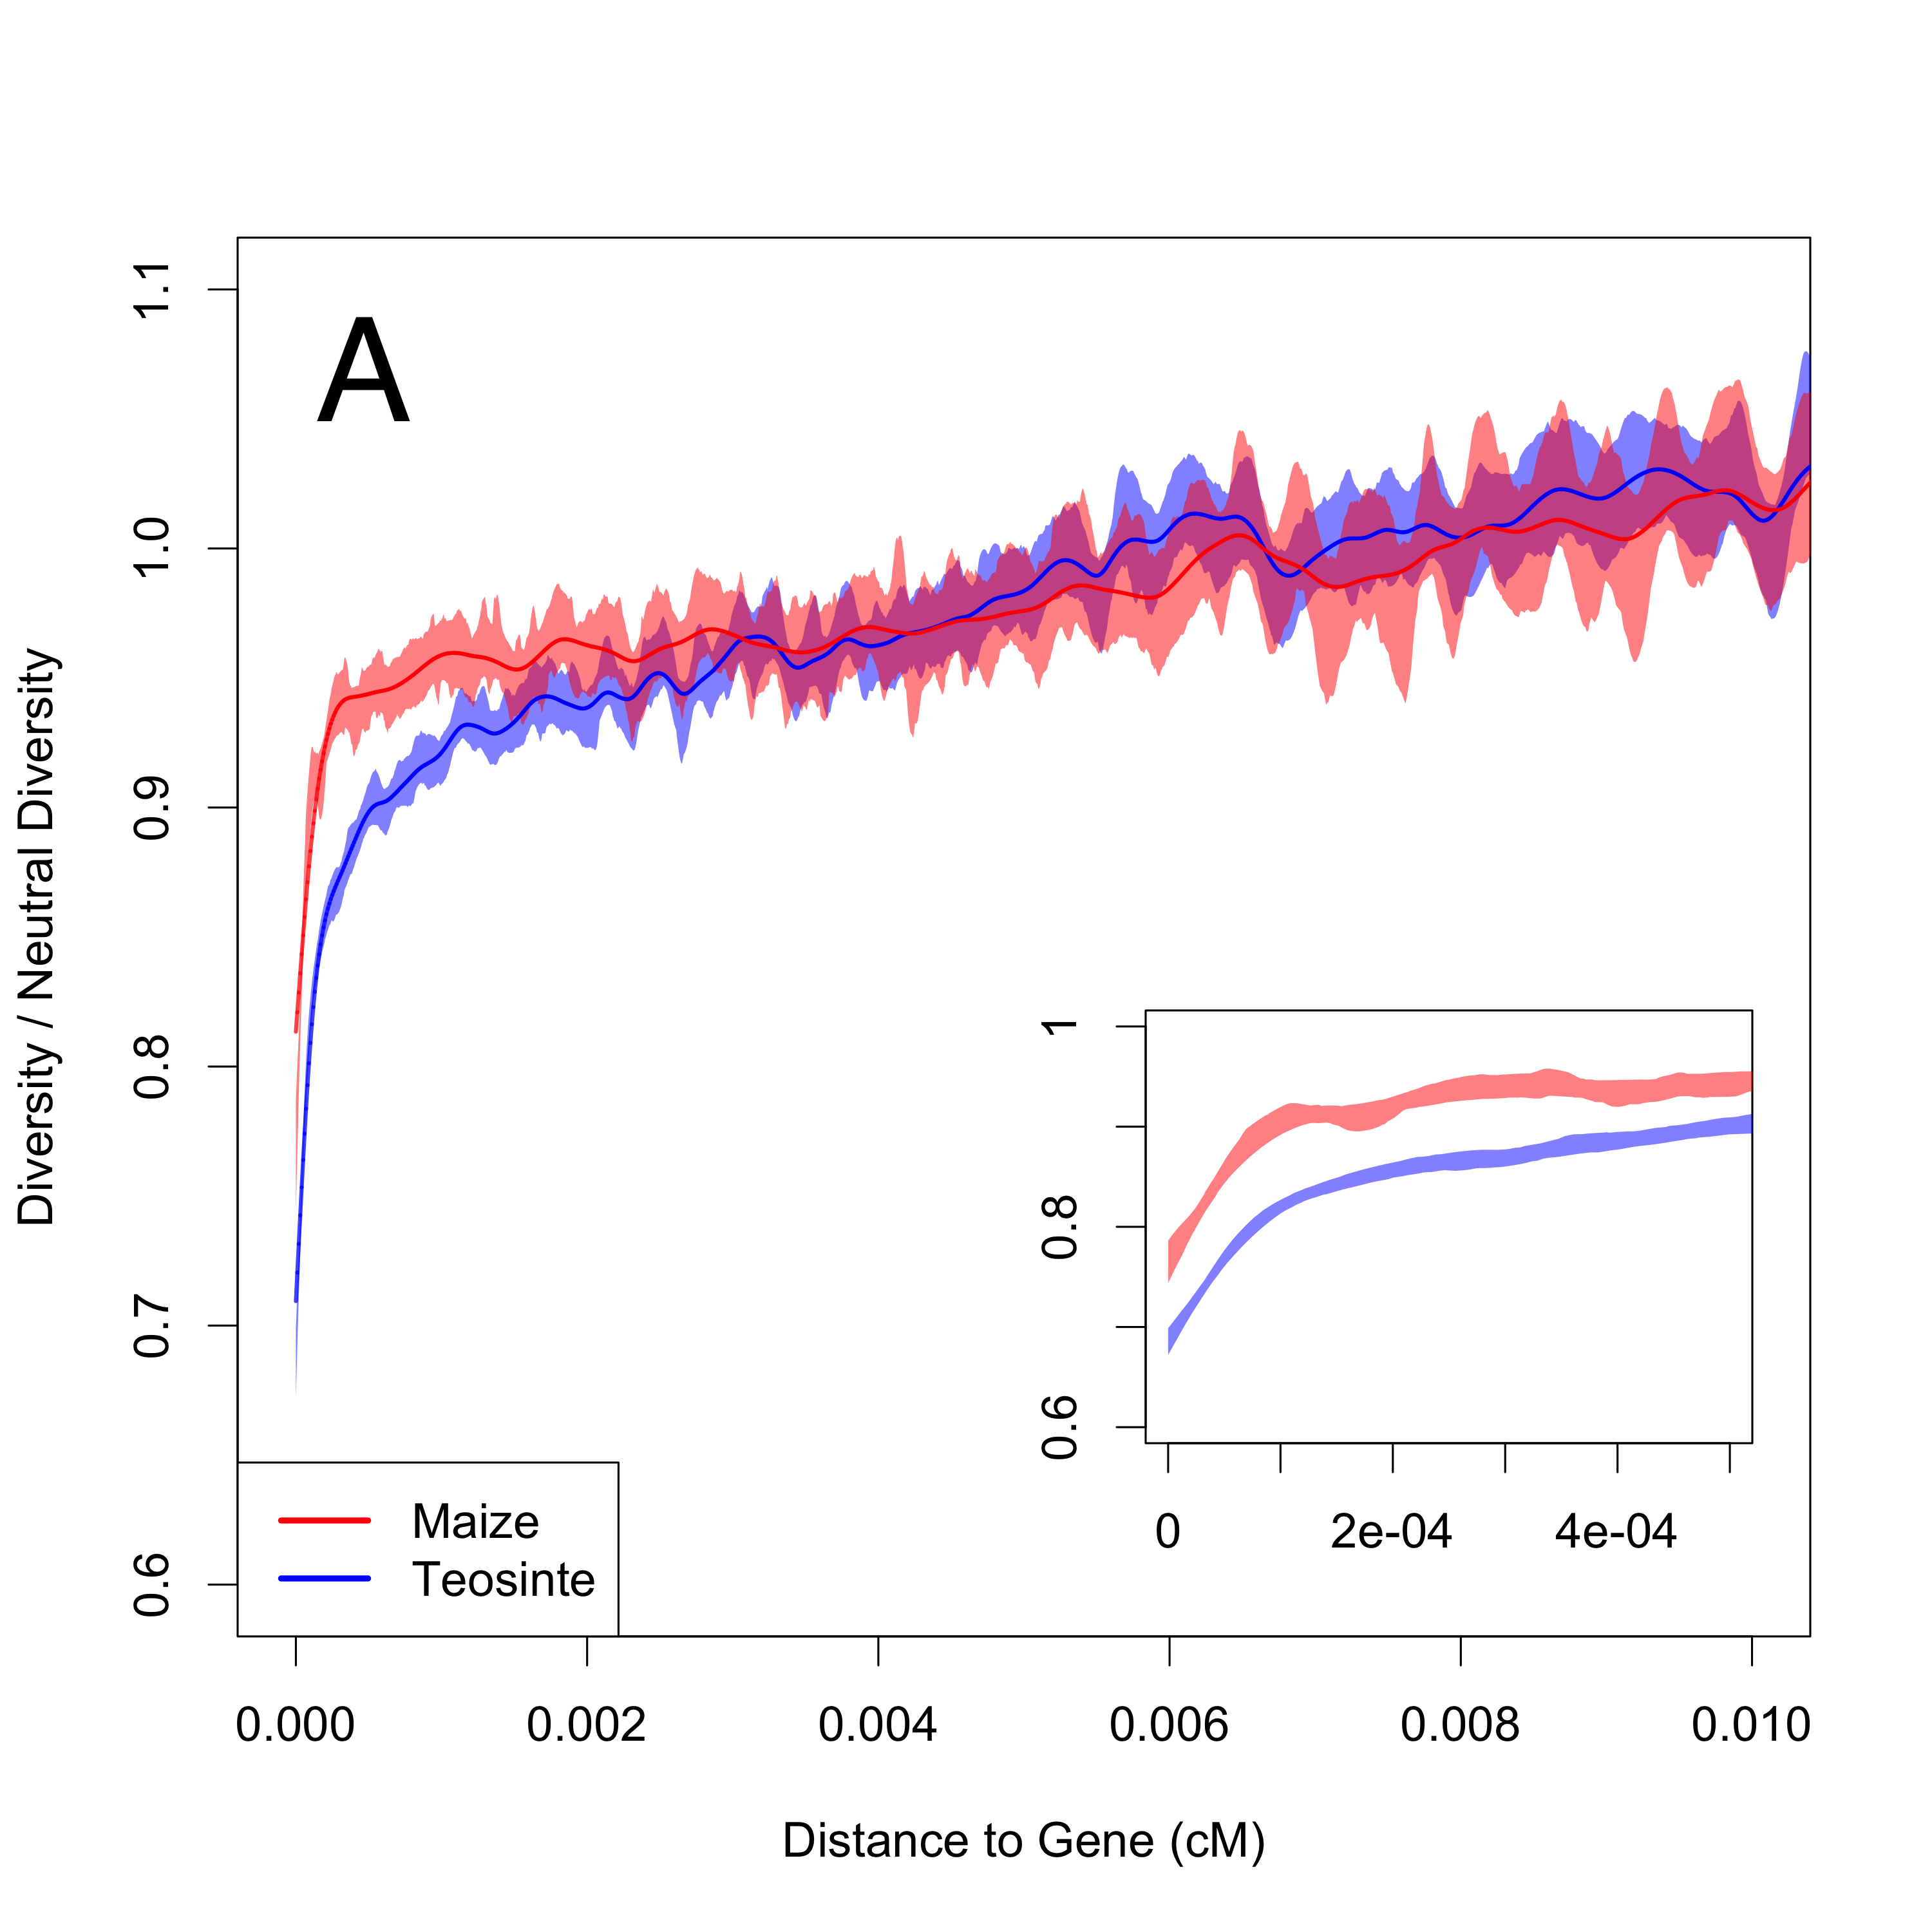
\includegraphics[width=.45\textwidth]{FigsAndFiles/distanceToGene_WithSignificance_Folded2_manuscript.png} 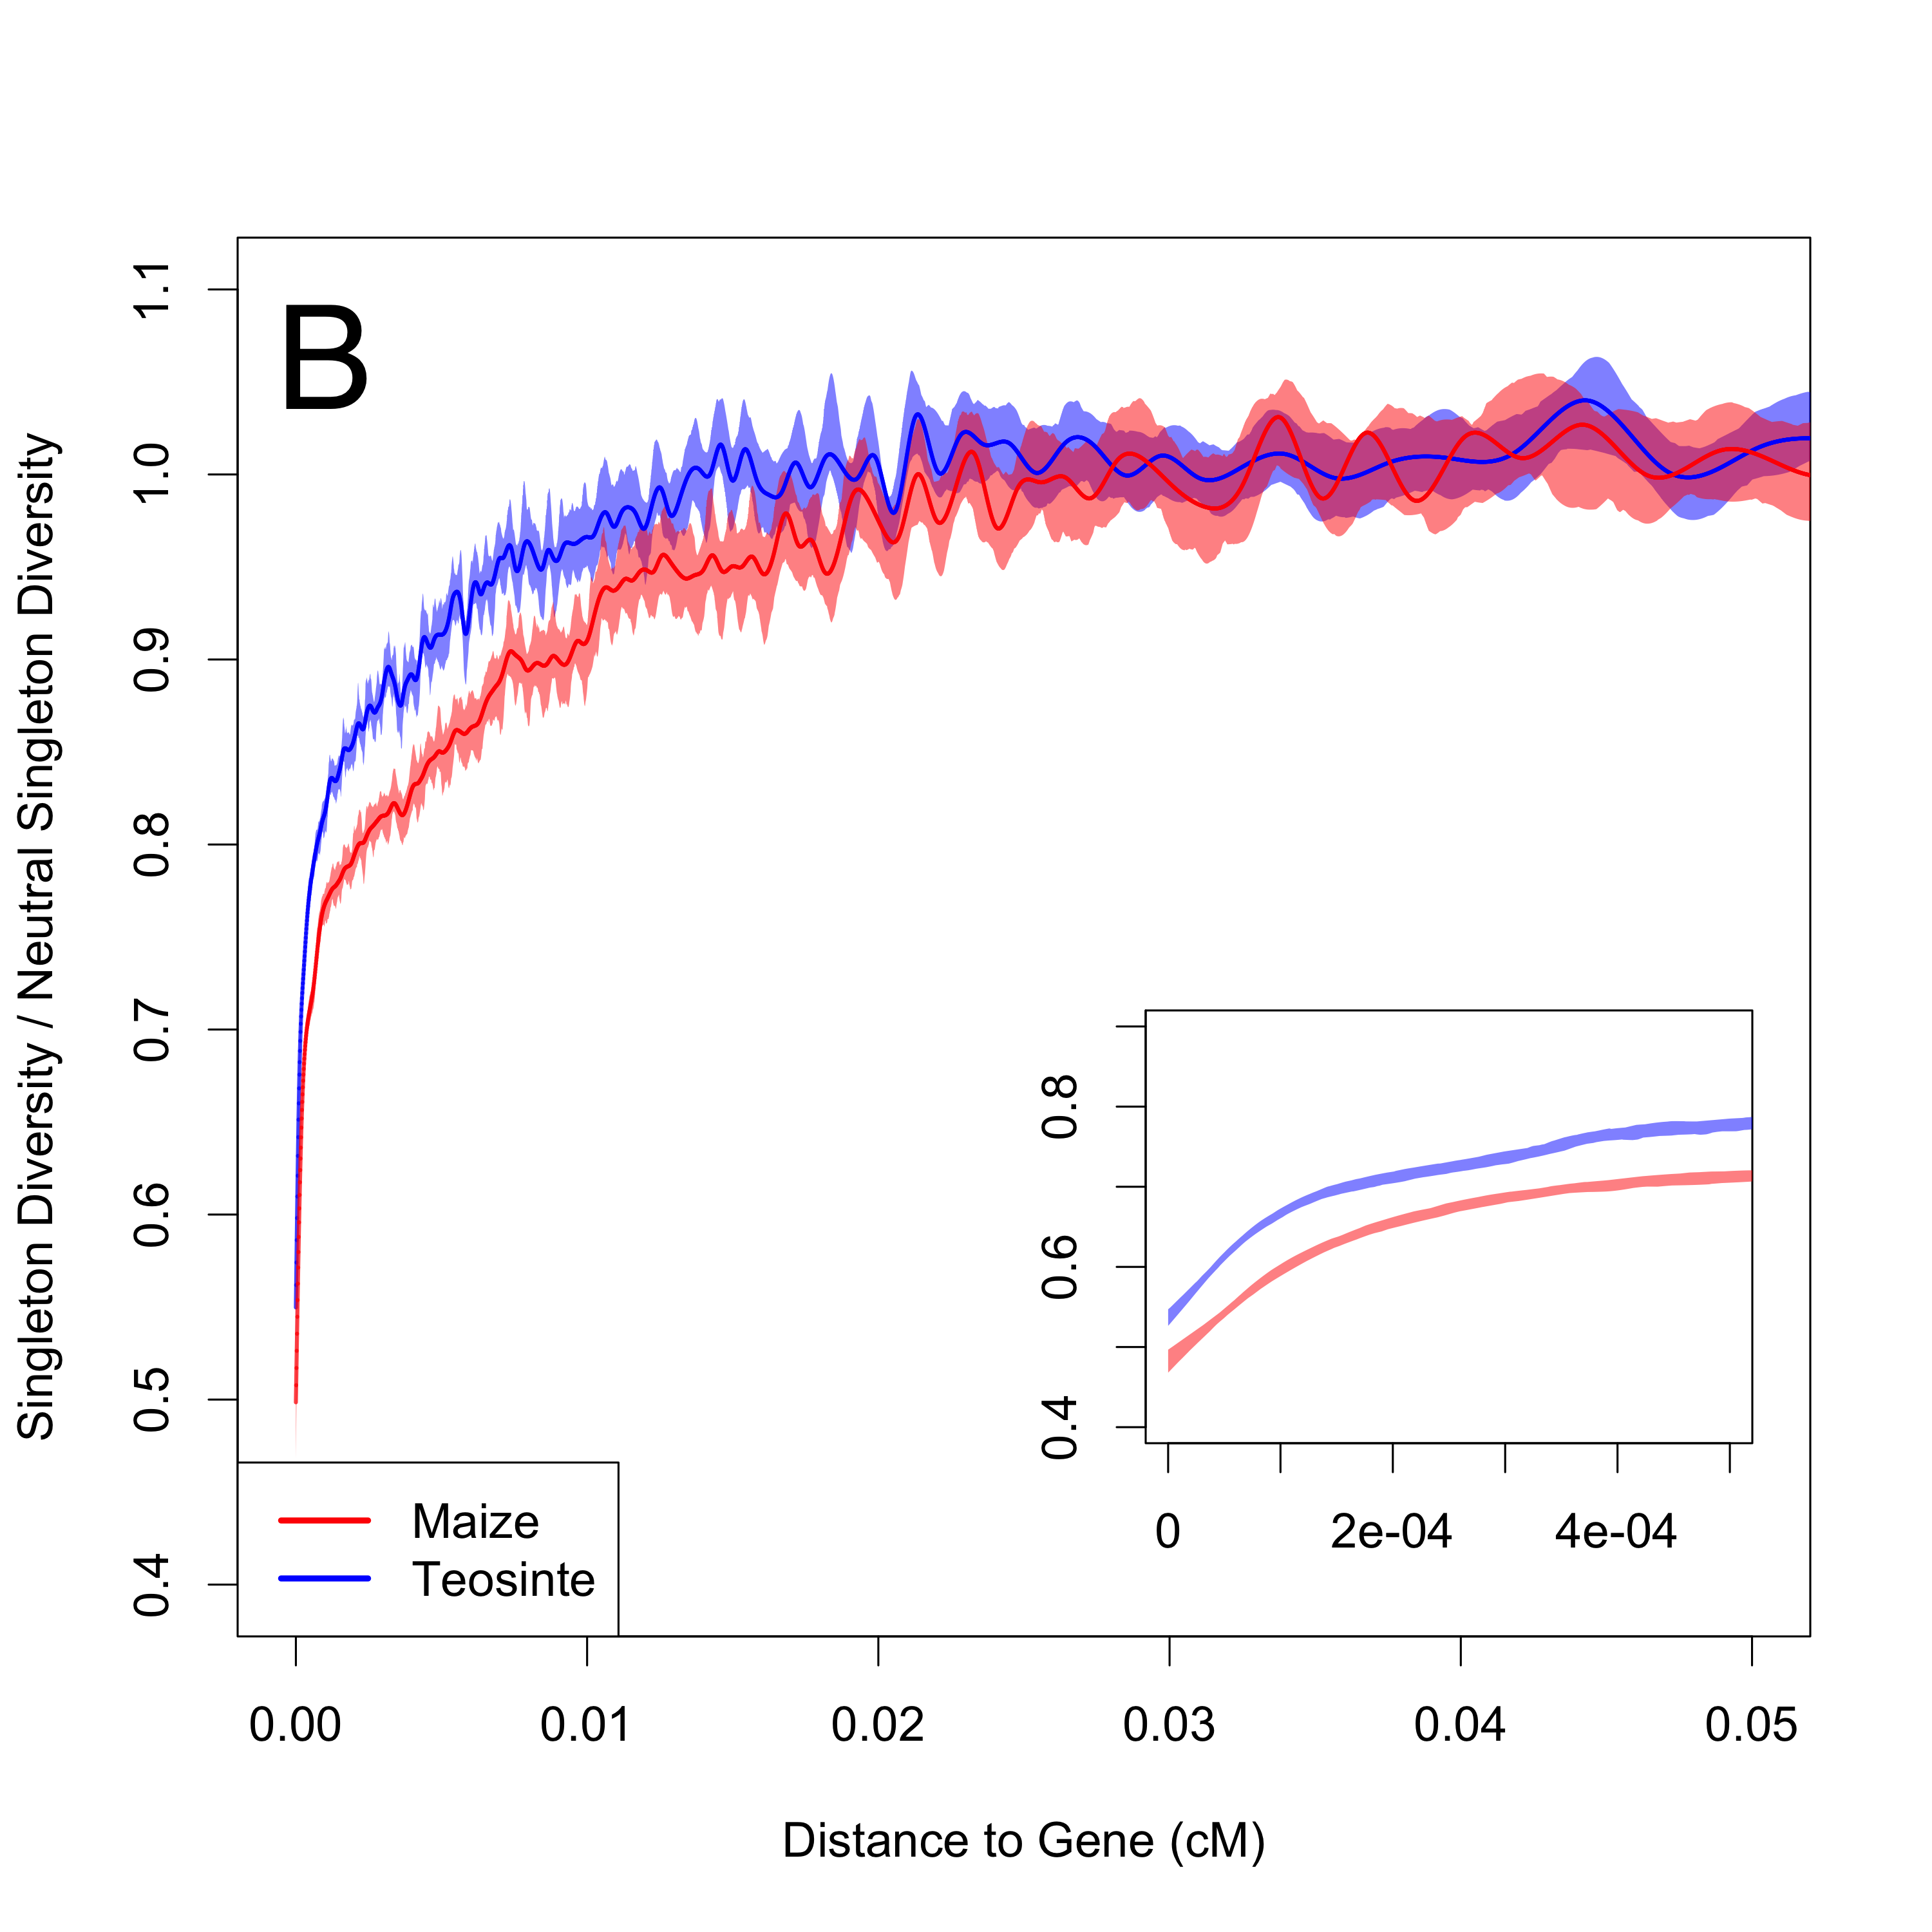
\includegraphics[width=.45\textwidth]{FigsAndFiles/distanceToGene_WithSignificance_Singletons_manuscript.png}
\caption{Relative level of diversity versus distance to the nearest
  gene, in maize and teosinte. Two measures of diversity were
  investigated. \textbf{A} displays pairwise
  diversity, which is most influenced by intermediate frequency
  alleles and therefore depicts more ancient evolutionary patterns,
  and \textbf{B} depicts singleton diversity, influenced by rare
  alleles and thus depicting evolutionary patterns in the recent past.}
\label{purify}
\end{figure*}


\textcolor{red}{This might be a good place to stick in a paragraph
  about curve fitting B to estimate s, mu.}

\subsection{Demography of maize domestication}
To explore whether differences in purifying selection between maize
and teosinte can be explained purely by demographic processes, we
first estimated the parameters of maize domestication using large-scale
sequencing data involving 23 inbred maize
landraces and 13 teosinte inbred lines included in the HapMap 2 panel
\cite{chia2012} \textcolor{red}{(supplemental table here)}. The maize
lines were collected from across the Americas and the teosinte lines
came from central Mexico. Before estimating demography, we compared
the site frequency spectrum (SFS) in genic and non-genic regions, and
observed substantial differences in the evolution of these classes of
sites. For both maize and teosinte, the SFS within genes showed a
dearth of low-frequency alleles and Tajima's D
\textcolor{red}{(reference here)} was therefore shifted
to more positive values \textcolor{red}{(figure here)}. This is consistent with the aforementioned purifying
selection and indicates that genic regions are not evolving
neutrally. Therefore, for demographic modeling we restricted analysis
to non-genic sites.

We used diffusion approximation as implemented in
dadi \cite{gutenkunst2009} to find the domestication parameters that best explain
the joint site frequency spectrum of maize and teosinte.  The model we optimized began with an
equilibrium ancestral population of size $N_a$
splitting into separate maize and teosinte populations $T_B$ generations in the past. Moving forward in
time from the split, teosinte maintained the ancestral population size, while
maize experienced an immediate effective population size change to
$N_b$ individuals, followed by exponential growth to size
$N_m$. Additionally, since the split a $M_{tm}$ individuals migrated
from teosinte into maize and $M_{mt}$ individuals migrated from maize
to teosinte.

The most likely model suggested an ancestral for $\theta$ ($4N\mu$) of
0.014734, which is similar to previous estimates
\textcolor{red}{(references here)}. Assuming a mutation rate of $\mu =
3 \times 10^{-8}$ \textcolor{red}{(reference here)}, this suggests an effective
population size of $N_a = 122,783$ individuals, a population split
$T_B = 15,523$ generations in the past, a maize bottleneck
effective populations size of $N_b = 6,455$ individuals (5.26\% of
$N_a$), a modern maize effective population size of $N_m = 366,973$
individuals, $M_{tm} = 1.35$ migrants per generation from teosinte to
maize, and $M_{mt} = 1.72$ migrants per generation from maize to
teosinte \textcolor{red}{(figure here)}. We note that a population
split over 15 thousand generations before present precedes estimates
from
archaeological data which suggests maize domestication began
approximately 9,000 years before present \textcolor{red}{(reference
  here)}. This could result from multiple generations per year, or in
may reflect teosinte population structure that was present before
domestication. Also, note that the genetic time of the population
split must precede morphological changes that could be identified
morphologically.   Additionally, because recent expansion is
most evidenced by rare alleles, and because these data provide low
power to detect rare alleles, we expect that the estimate of  $N_m =
366,973$, or $\sim 3N_a$, is likely an underestimate. \textcolor{red}{(This
  is where evaluation using Kate's SFS should go)}.


\section{Discussion}
\subsection{Discussion 1}
Text goes here

\subsection{Discussion 2}
Text goes here

\begin{materials}
\subsection{Plant materials}
Accessions studied were selected from the Maize HapMap2
panel \cite{chia2012} . Principal component analysis was employed to ensure that
closely related individuals were not included due to their potential
to bias results \textcolor{red}{(maybe a supplemental figure here)}. Ultimately, 23 maize inbreds derived from a diverse
assortment of landraces were selected for inclusion. Thirteen teosinte
inbred lines, all members of the subspecies Z. \emph{mays}
ssp. \emph{parviglumis}, were utilized. Sequences were mapped to the
maize B73 version 3 reference genome \cite{schnable2009}
(ftp://ftp.ensemblgenomes.org/pub/plants/release-22/fasta/zea\_mays/dna/).

\subsection{Interpolating genetic position}
For many of the following analyses, physical position along a
chromosome was a less relevant measure of map location than was genetic
position. Therefore, physical positions were converted to genetic
positions by interpolating from the NAM genetic map (REFERENCE), which
provides a 1 cM resolution for physical to genetic conversion. Within
R \cite{R2014}, physical positions with corresponding genetic positions in
the NAM map were used as anchors. Physical positions in our dataset
wihout corresponding genetic position were assigned genetic positions by scaling
the anchored genetic positions according to the physical distance
between the unlabeled position and the flanking anchors.

\subsection{Estimating the site frequency spectrum}
To estimate individual  and joint site frequency spectra (SFS) for
maize and teosinte from inbred lines, each inbred individual was treated as representing
a single haplotype from its population. These were
separately computed for genic and intergenic regions, as well as for
the whole genome together. First, genic and intergenic regions were isolated using
the biomaRt package \cite{durinck2009,durinck2005} of R \cite{R2014}. Genic
regions were defined as DNA between the start and stop position of a
gene, while intergenic regions were required to be at least 5kb up- or
down-stream from a gene start/stop. With regions defined, SFS were
estimated with ANGSD \cite{korneliussen2014}. Individual population SFS were
estimated using all positions observed in at least 80\% of the
individuals in the population, and joint SFS were estimated using all
positions observed in at least 80\% of individuals in both
populations. Individuals were
assumed to be fully inbred (-doSaf 2), and subsequently allele frequencies were
divided by two to indicate haplotype frequencies. Quality filters were
employed such that reads with quality score below 30 and bases with
quality score below 20 were discarded (-minMapq 30 and -minQ 20), as were reads that didn't map
uniquely (-uniqueOnly 0). Quality scores around indels were adjusted
as in Samtools (-baq 0). Genotype likelihoods were estimated using the samtools
method (-GL 1). Major and minor alleles were inferred from the data
(-doMaf 1). Because ANGSD cannot calculate a folded joint SFS, the
maize reference genome was used for polarization and then unfolded spectra
were folded using dadi \cite{gutenkunst2009}.

\subsection{Demographic inference}

\subsection{Evaluating diversity around substitutions}
To investigate diversity around substitutions, maize and teosinte pairwise diversity was first
calculated in 1,000 kb non-overlapping windows using ANGSD
\cite{korneliussen2014}. This was performed separately for both maize and
teosinte, using the same filters as employed for estimating the
SFS. Next, SNPs and genotypes among maize, teosinte, and tripsicum were called. Tripsicum bam files
were downloaded from (TRIPSICUM FILES), and then all SNPs with a
p-value less than 1e-6 were called using ANGSD. Quality filters were
as the same as before, and genotypes were only called when the
posterior probability was above 0.95. From the set of called SNPs and
genotypes, substitutions between maize and tripsicum, as well as
between teosinte and tripsicum were identified using R \cite{R2014} as all positions with
no more than 20\% missing data for which every maize or teosinte
allele differed from the observed tripsicum allele. At each class of
substitution, effects were estimated using the ensembl variant effects
predictor \cite{mclaren2010}.

For each diversity window with at least 100 bps observed, the distance from the window center to the
nearest synonymous and nonsynonymous (missense) substitution was
computed. Then, following the methods of \cite{hernandez2011}, a loess
curve was plotted for diversity values against the distance to the
nearest synonymous or nonsynonymous substitution. A span of 0.01 was
utilized. Unlike
\cite{sattath2011}, we did not fit separate loess curves in the up- and
down-stream directions, but instead fit single curves encompassing
both directions.

\subsection{Evaluating diversity around genes and conserved sequences}
Two types of diversity surrounding genes were investigated. The first
was pairwise diversity in 1kb windows, as described previously. The
second was singleton diversity in 1kb windows. Singletons represent
the rarest class of alleles that this dataset can identify, and
collectively demonstrate the most recent patterns of evolution. Minor
allele frequencies were estimated with ANGSD \cite{korneliussen2014} using the
same quality filters previously described. Then, the number of
singletons in each non-overlapping 1kb window was calculated with R
\cite{R2014}. BiomaRt \cite{durinck2009, durinck2005} was then used to identify
the center of each gene. Next, the distance from each diversity window
to the nearest gene center was computed. Teosinte diversity is
generally higher then maize diversity. Therefore, to enable comparisons between
the reduction of diversity around genes in maize and teosinte, a
neutral measure of pairwise and singleton diversity for each taxa was estimated according to
mean pairwise and singleton diversity at windows greater than 0.01 cM from the nearest
gene. Then, pairwise and singleton diversity at each window was
standardized by dividing by the corresponding neutral
measure. Separately for pairwise and singleton diversity in maize and
teosinte, cubic smoothing splines were fit to
describe diversity levels according to the distance to the nearest
gene. Significant differences were assessed by taking 100 bootstrap
samples and re-fitting the cubic smoothing spline to each. Then, the
2.5\% and 97.5\% quantiles of values along the bootstrapped splines
were identified.

\subsection{Simulations}

\end{materials}

\begin{acknowledgments}
Various thankyous will be in order.
\end{acknowledgments}


% \begin{thebibliography}{10}
% \bibitem{dadi}
% R.~Gutenkunst, R.~Hernandez,S.~Williamson, and C.~Bustamante, {\em
%   Inferring the joint demographic history of multiple populations from
%   multidimensional SNP frequency data}, PLoS Genetics., 5:10 (2009), e1000695.

% \bibitem{hapmap2}
% J.~Chia, C.~Song, P.~Bradbury, D.~Costich, N.~de~Leon, and others,
% \emph{Maize HapMap2 identifies extant variation from a genome in
%   flux}, Nature Genetics., 44 (2012), 803-807.

% \bibitem{maizeGenome}
% P.~Schnable, D.~Ware, R.~Fulton, J.~Stein, F.~Wei, \emph{The B73 maize
% genome:complexity, diversity, and dynamics}, Science., 326:5956
% (2009), 1112-1115.

% \bibitem{angsd}
% T.~Korneliussen, A.~Albrechtsen, and R.~Nielsen, \emph{ANGSD: Analysis of
% next generation sequencing data}, BMC Bioinformatics., 15:356 (2014),
% 10.1186/s12859-014-0356-4.

% \bibitem{R}
% R Core Team, \emph{R: A language and environment for statistical
%   computing}, R Foundation for Statistical Computing., Vienna,
% Austria.

% \bibitem{biomaRt1}
% S.~Durinck, P.T.~Soekknabm E.~Birney, and W.~Huber, \emph{Mapping
%   identifiers for the integration of genomic datasets with the
%   R/Bioconductor package biomaRt}, Nature Protocols., 4 (2009),
% 1184-1191.

% \bibitem{biomaRt2}
% S.~Durinck, Y.~Moreau, A.~Kasprzyk, S.~Davis, B.~De~Moor, and others,
% \emph{BioMart and Bioconductor: a powerful link between biological
%   databases and microarray data analysis}, Bioinformatics, 21 (2005),
% 3439-3440.

% \bibitem{vep}
% W.~McLaren, B.~Pritchard, D.~Rios, Y.~Chen, P.~Flicek, and
% F.~Cunningham, \emph{Deriving the consequences of genomic variants
%   with the Ensembl API and SNP Effect Predictor}, Bioinformatics,
% 26:16 (2010), 2069-2070.

% \bibitem{hernandez11}
% R.D.~Hernandez, J.L.~Kelley, E.~Elyashiv, S.C.~Melton, A.~Auton, and
% others, \emph{Classic selective sweeps were rare in recent human
%   evolution}, Science, 331:6019 (2011), 920-924.

% \bibitem{sattath11}
% S.~Sattath, E.~Elyashiv, O.~Kolodny, Y.~Rinott, and G.~Sella,
% \emph{Pervasive adaptative protein evolution apparent in diversity
%   patterns around amino acid substitutions in Drosophila simulans},
% PLoS Genetics, 7:2 (2011), e1001302.

% \bibitem{charlesworth93}
% B.~Charlesworth, M.~T.~Morgan, and D.~Charlesworth, \emph{The Effect
%   of Deleterious Mutations on Neutral Molecular Variation}, Genetics,
% 134 (1993), 1289-1303.

% \end{thebibliography}

\bibliography{Reference}
\bibliographystyle{pnas}
%\nocite{*}


\end{article}
\end{document}